\documentclass[5pt]{article}
\usepackage{multicol,multirow}
\usepackage{graphicx} % Required for inserting images
\usepackage[margin=0.75cm]{geometry}
\usepackage{xcolor}
\usepackage{amsmath}
\usepackage{mathtools}
\usepackage{relsize}

\usepackage[english]{babel}
\newtheorem{theorem}{Theorem}

\usepackage{empheq}
\usepackage{amsfonts}

\usepackage{tkz-euclide}
\usepackage{tikz}

\definecolor{LightGray}{gray}{0.9}

\usepackage{minted}

\DeclarePairedDelimiter\abs{\lvert}{\rvert}%
\DeclarePairedDelimiter\norm{\lVert}{\rVert}%

\makeatletter
\let\oldabs\abs
\def\abs{\@ifstar{\oldabs}{\oldabs*}}

\newcommand{\tr}[3]{
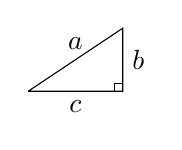
\begin{tikzpicture}[scale=0.40]
    \coordinate [] (A) at (-1.5cm,-1.cm);
    \coordinate [] (C) at (1.5cm,-1.0cm);
    \coordinate [] (B) at (1.5cm,1.0cm);
    \draw (A) -- node[above] {$a$} (B) -- node[right] {$b$} (C) -- node[below] {$c$} (A);
    \draw (1.25cm,-1.0cm) rectangle (1.5cm,-0.75cm);
\end{tikzpicture}
}


\begin{document}


\begin{center}
     \Large{\textbf{Discrete Mathematics}}\\
     \small{Class: MATH 2410}\hfill\small{\textcopyright Maximilien Notz \the\year{}}
     \noindent\rule{20.2cm}{0.4pt}
\end{center}


\begin{multicols}{2}
\setcounter{secnumdepth}{0}

%%%%%%%%%%%%%%%%%%%%
%% CODE %%%%%%%%%%%%
%%%%%%%%%%%%%%%%%%%%

\subsection{Naive Set Theory}
\subsubsection{Set Notation}
\begin{tabular}{ll}







    Cartesian Product & $A\times B=\{(x,y)|x\in A\land y \in B\}$
    
\end{tabular}

\subsection{Functions}

\begin{tabular}{ll}
    Functions           & A rule that assigns each input exactly one \\
                        & output.\\
    Range               & The set of all elements which are assigned to at\\
                        & least one element of the domain by the function.\\
    Domain              & The set of all input of a function.\\
    Codomain            & The set of all allowable output a function.\\
    $f:x\leftarrow y$   & a function $f$ with a domain $x$ and a codomain $y$.\\
    Recursive f.        & \\
    Injectiuve          & every element of the codomain is the image  of \\
                        & \textbf{at most} one element from the domain.\\
    Surjective          & every element of the codomain is the image  of \\
                        & \textbf{at least} one element from the domain.\\
    Bijection           & A function that is \textbf{Injective} and \textbf{Surjective}.\\
    Image               & $f(A)=\{f(a)\in Y: a\in A\}$, where $A\subset\text{domain}$.\\
    Inverse Image       & $f^{-1}(B)=\{f(b)\in X: b\in B\}$, where \\
                        & $B\subset\text{codomain}$.\\
\end{tabular}

\subsection{Counting}
\subsubsection{Additive Principle}
\textbf{General Definition:} 
if event $A$ can occur in $m$ ways, and even $B$ can occur in $n$ \textbf{disjoint} ($A$ and $B$ can't apen at the same time.) ways, then $A$ and $B$ can occur in $m+n$ ways.\\   
\textbf{Set Definition:} Given 2 sets $A$ and $B$, if $A\cap B =\emptyset$, then $|A\cap B| = |A| + |B|$.


\subsubsection{Multiplicative Principle}
\textbf{General Definition:} if event $A$ can occur $m$ ways, and each possibility for $A$ allows for exactly $n$ ways for event $B$, then the event "$A$ and $B$" can occur $m\cdot n$ ways.\\
\textbf{Set Definition:} Given 2 sets $A$ and $B$, we have $|A\times B|=|A|\cdot|B|$.


\subsection{Sequences}

\subsection{Symbolic Logic}

\subsection{Proofs}

\subsection{Graph Theory}



\end{multicols}
\end{document}